%! alt A cube of side 2 in parallel projection, with its hidden edges dashed and its centre K = (1, 1, 1) marked. The plane through K normal to (1, 1, 1) cuts the cube in a shaded regular hexagon whose vertices are the six edge midpoints (2, 0, 1), (2, 1, 0), (1, 2, 0), (0, 2, 1), (0, 1, 2) and (1, 0, 2). Its three long diagonals pass through K and are three of the thirteen lines through K: the lines in directions (1, -1, 0), (0, 1, -1) and (1, 0, -1). Opposite vertices of the hexagon are symmetric about K.
%! after_paragraph 5
%! scale 13/5
% The shared preamble of every Cevian figure. pipeline/figures turns these colours into theme-aware paint,
% and refuses any other colour, so draw only with them:
%   figink (lines and labels), figaux (construction lines), figaccent (the object the argument turns on),
%   figtint and figaccenttint (light fills).
\documentclass[border=1.5pt]{standalone}
\usepackage{tkz-euclide}
\definecolor{figink}{RGB}{0,0,0}
\definecolor{figaux}{RGB}{85,85,85}
\definecolor{figaccent}{RGB}{192,57,43}
\definecolor{figtint}{RGB}{221,221,221}
\definecolor{figaccenttint}{RGB}{245,213,208}
% tkz-euclide's defaults draw circles, compasses and marks in 50% grey and fill points with a tint.
\makeatletter
\def\tkz@otherlinecolor{figink}
\def\tkz@euc@circlecolor{figink}
\def\tkz@euc@compasscolor{figink}
\def\tkz@euc@mkcolor{figink}
\def\tkz@mk@fill{figink}
\def\tkz@euc@pointfillcolor{figink}
\makeatother
\tkzSetUpLine[color=figink,line width=.7pt]
\tkzSetUpArc[color=figink,line width=.7pt]
\tkzSetUpCompass[color=figink,line width=.5pt]
\tkzSetUpPoint[color=figink,fill=figink,size=3.1pt]
\tikzset{
  every picture/.style={line cap=round,line join=round,color=figink},
  circle style/.append style={color=figink,line width=.7pt},
  aux/.style={color=figaux,line width=.45pt,dash pattern=on 2.6pt off 2pt},
  key/.style={color=figaccent,line width=1pt},
  mk/.style={color=figink,line width=.5pt},
  lbl/.style={color=figink,inner sep=2.2pt},
  len/.style={color=figink,inner sep=1.5pt,font=\small},
}

\begin{document}
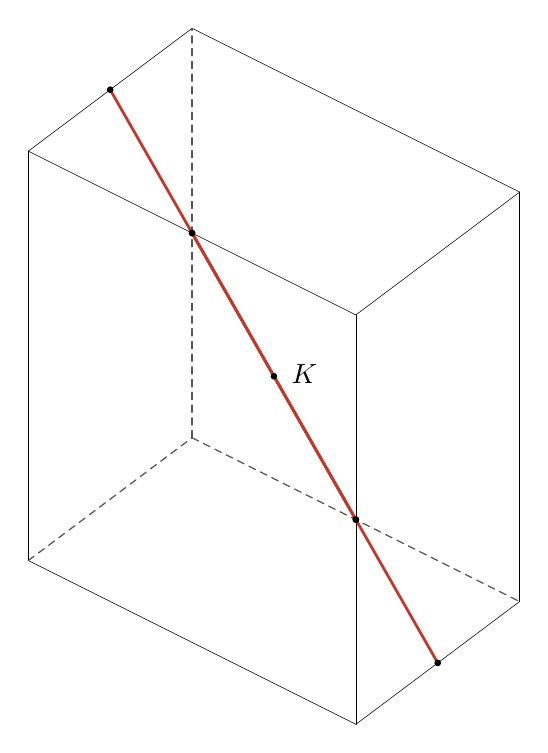
\begin{tikzpicture}
\tkzDefPoint(0.0,0.0){V000} %! V000 = (4/5*0 + 2/5*0, -2/5*0 + 3/10*0 + 0)
\tkzDefPoint(0.0,5.2000000){V002} %! V002 = (4/5*0 + 2/5*0, -2/5*0 + 3/10*0 + 2)
\tkzDefPoint(2.0800000,1.5600000){V020} %! V020 = (4/5*0 + 2/5*2, -2/5*0 + 3/10*2 + 0)
\tkzDefPoint(2.0800000,6.7600000){V022} %! V022 = (4/5*0 + 2/5*2, -2/5*0 + 3/10*2 + 2)
\tkzDefPoint(4.1600000,-2.0800000){V200} %! V200 = (4/5*2 + 2/5*0, -2/5*2 + 3/10*0 + 0)
\tkzDefPoint(4.1600000,3.1200000){V202} %! V202 = (4/5*2 + 2/5*0, -2/5*2 + 3/10*0 + 2)
\tkzDefPoint(6.2400000,-0.52000000){V220} %! V220 = (4/5*2 + 2/5*2, -2/5*2 + 3/10*2 + 0)
\tkzDefPoint(6.2400000,4.6800000){V222} %! V222 = (4/5*2 + 2/5*2, -2/5*2 + 3/10*2 + 2)
\tkzDefPoint(4.1600000,0.52000000){V201} %! V201 = (4/5*2 + 2/5*0, -2/5*2 + 3/10*0 + 1)
\tkzDefPoint(5.2000000,-1.3000000){V210} %! V210 = (4/5*2 + 2/5*1, -2/5*2 + 3/10*1 + 0)
\tkzDefPoint(4.1600000,0.52000000){V120} %! V120 = (4/5*1 + 2/5*2, -2/5*1 + 3/10*2 + 0)
\tkzDefPoint(2.0800000,4.1600000){V021} %! V021 = (4/5*0 + 2/5*2, -2/5*0 + 3/10*2 + 1)
\tkzDefPoint(1.0400000,5.9800000){V012} %! V012 = (4/5*0 + 2/5*1, -2/5*0 + 3/10*1 + 2)
\tkzDefPoint(2.0800000,4.1600000){V102} %! V102 = (4/5*1 + 2/5*0, -2/5*1 + 3/10*0 + 2)
\tkzDefPoint(3.1200000,2.3400000){V111} %! V111 = (4/5*1 + 2/5*1, -2/5*1 + 3/10*1 + 1)
%! fact midpoint(V111, V201, V021)
%! fact midpoint(V111, V210, V012)
%! fact midpoint(V111, V120, V102)
%! fact midpoint(V111, V000, V222)
%! fact parallel(V201, V210, V021, V012)
%! fact parallel(V210, V120, V012, V102)
%! fact parallel(V120, V021, V102, V201)
%! fact midpoint(V201, V200, V202)
%! fact midpoint(V021, V020, V022)
\tkzFillPolygon[color=figaccenttint](V201,V210,V120,V021,V012,V102)
\tkzDrawSegments(V000,V200 V200,V202 V202,V002 V002,V000 V200,V220 V220,V222 V222,V202 V002,V022 V022,V222)
\tkzDrawSegments[aux](V000,V020 V020,V220 V020,V022)
\tkzDrawPolygon(V201,V210,V120,V021,V012,V102)
\tkzDrawSegments[key](V201,V021 V210,V012 V120,V102)
\tkzDrawPoints(V201,V210,V120,V021,V012,V102,V111)
\tkzLabelPoint[xshift=11pt,yshift=6.5pt,lbl](V111){$K$}
\end{tikzpicture}
\end{document}
